% ============================================================
%   PROYECTO INSTRUMENTACION FINAL
%   Sistema de Control e Instrumentación para una Columna de Absorción
%   ESIQIE — Instituto Politécnico Nacional
%   Grupo 5IV81, Equipo 4 — Mayo 2026
% ============================================================

\documentclass[12pt,letterpaper]{article}

% ------- CODIFICACIÓN Y LENGUAJE -------
\usepackage[utf8]{inputenc}
\usepackage[T1]{fontenc}
\usepackage[spanish,es-tabla]{babel}

% ------- GEOMETRÍA -------
\usepackage[
  top=2.5cm, bottom=2.5cm,
  left=3cm,  right=2.5cm,
  headheight=15pt
]{geometry}

% ------- TIPOGRAFÍA Y COLORES -------
\usepackage{lmodern}
\usepackage{xcolor}
\definecolor{ipnguinda}{RGB}{110,0,25}
\definecolor{ipngold}{RGB}{204,153,0}
\definecolor{azulacero}{RGB}{30,80,130}
\definecolor{grisclaro}{RGB}{245,245,245}
\definecolor{grisnota}{RGB}{100,100,100}

% ------- GRÁFICOS Y TABLAS -------
\usepackage{graphicx}
\usepackage{float}
\usepackage{booktabs}
\usepackage{longtable}
\usepackage{array}
\usepackage{tabularx}
\usepackage{multirow}
\usepackage{colortbl}

% ------- ENCABEZADO Y PIE -------
\usepackage{fancyhdr}
\usepackage{lastpage}

% ------- SECCIONES Y FORMATO -------
\usepackage{titlesec}
\usepackage{tocloft}
\usepackage{enumitem}
\usepackage{parskip}
\usepackage{microtype}

% ------- CAJAS Y MARCOS -------
\usepackage{tcolorbox}
\tcbuselibrary{skins, breakable}

% ------- HIPERVÍNCULOS -------
\usepackage[
  colorlinks=true,
  linkcolor=ipnguinda,
  urlcolor=azulacero,
  citecolor=azulacero,
  pdftitle={PROYECTO INSTRUMENTACION FINAL},
  pdfauthor={Equipo 4 - Grupo 5IV81 - ESIQIE IPN},
  pdfsubject={Sistema de Control e Instrumentacion para Columna de Absorcion},
  pdfkeywords={instrumentacion, columna de absorcion, ESIQIE, IPN, control de procesos}
]{hyperref}

% ------- CONFIGURACIÓN DE SECCIONES -------
\titleformat{\section}
  {\Large\bfseries\color{ipnguinda}}
  {\thesection.}{0.7em}{}
  [{\color{ipnguinda}\rule{\textwidth}{1.2pt}}]

\titleformat{\subsection}
  {\large\bfseries\color{azulacero}}
  {\thesubsection.}{0.6em}{}
  [{\color{azulacero!60!black}\rule{\textwidth}{0.5pt}}]

\titleformat{\subsubsection}
  {\normalsize\bfseries\color{azulacero!80!black}}
  {\thesubsubsection.}{0.5em}{}

\titlespacing{\section}{0pt}{18pt}{8pt}
\titlespacing{\subsection}{0pt}{14pt}{6pt}
\titlespacing{\subsubsection}{0pt}{10pt}{4pt}

% ------- ENCABEZADO / PIE DE PÁGINA -------
\pagestyle{fancy}
\fancyhf{}
\fancyhead[L]{\small\color{grisnota}\textit{Sistema de Control — Columna de Absorción}}
\fancyhead[R]{\small\color{grisnota}\textit{ESIQIE — IPN}}
\fancyhead[C]{\color{ipnguinda}\rule[-2pt]{0pt}{10pt}}
\renewcommand{\headrulewidth}{0.4pt}
\renewcommand{\headrule}{\color{ipnguinda}\hrule width\headwidth height\headrulewidth}
\fancyfoot[C]{\small\thepage\ de \pageref{LastPage}}
\fancyfoot[R]{\small\color{grisnota}Equipo 4 — Grupo 5IV81}

% ------- CAJA DE ESPECIFICACIONES -------
\newtcolorbox{especbox}[1][]{
  enhanced, breakable,
  colback=grisclaro,
  colframe=ipnguinda,
  fonttitle=\bfseries\color{white},
  coltitle=white,
  attach boxed title to top left={yshift=-2mm, xshift=4mm},
  boxed title style={colback=ipnguinda, rounded corners},
  rounded corners, arc=4pt,
  #1
}

\newtcolorbox{notabox}[1][]{
  enhanced,
  colback=azulacero!8,
  colframe=azulacero,
  left=6pt, right=6pt, top=4pt, bottom=4pt,
  rounded corners, arc=3pt,
  #1
}

% ------- TABLA GRIS ALTERNADO -------
\newcolumntype{L}[1]{>{\raggedright\arraybackslash}p{#1}}
\newcolumntype{C}[1]{>{\centering\arraybackslash}p{#1}}

% ------- SEPARACIÓN DE PÁRRAFOS -------
\setlength{\parindent}{0pt}
\setlength{\parskip}{6pt}

% ============================================================
\begin{document}
% ============================================================

% ============================================================
%  PORTADA
% ============================================================
\begin{titlepage}
\thispagestyle{empty}
\pagecolor{white}

% Franja superior guinda
\noindent\colorbox{ipnguinda}{%
  \begin{minipage}{\dimexpr\linewidth+2\fboxsep}
    \vspace{6pt}
    \centering\color{white}\small
    \textbf{INSTITUTO POLITÉCNICO NACIONAL}
    \vspace{6pt}
  \end{minipage}%
}

\vspace{4pt}

% Logos institucionales
\begin{minipage}[c]{0.28\linewidth}
  \centering
  
\includegraphics[width=3.2cm]{figuras/logo_ipn.png}
\end{minipage}
\hfill
\begin{minipage}[c]{0.42\linewidth}
  \centering
  {\large\bfseries\color{ipnguinda} Instituto Politécnico Nacional}\\[3pt]
  {\normalsize\bfseries Escuela Superior de Ingeniería}\\
  {\normalsize\bfseries Química e Industrias Extractivas}\\[2pt]
  {\small Academia de Diseño e Ingeniería de Apoyo}
\end{minipage}
\hfill
\begin{minipage}[c]{0.22\linewidth}
  \centering
  
\includegraphics[width=2.8cm]{figuras/logo_esiqie.png}
\end{minipage}

\vspace{4pt}
{\color{ipnguinda}\rule{\linewidth}{1.5pt}}

\vspace{1.2cm}

\begin{center}

{\large\bfseries\color{grisnota} MATERIA:}\\[4pt]
{\Large\bfseries\color{azulacero} INSTRUMENTACIÓN INDUSTRIAL}\\[0.8cm]

{\color{ipnguinda}\rule{0.55\linewidth}{0.8pt}}\\[0.6cm]

{\fontsize{22}{28}\selectfont\bfseries\color{ipnguinda}
  SISTEMA DE CONTROL E INSTRUMENTACIÓN\\[6pt]
  PARA UNA COLUMNA DE ABSORCIÓN
}\\[0.5cm]

{\color{ipnguinda}\rule{0.55\linewidth}{0.8pt}}\\[1cm]

% Caja de integrantes
\begin{tcolorbox}[
  enhanced,
  colback=grisclaro,
  colframe=ipnguinda,
  width=0.82\linewidth,
  arc=6pt,
  boxrule=1.2pt,
  title={\bfseries\color{white} INTEGRANTES},
  attach boxed title to top center={yshift=-2mm},
  boxed title style={colback=ipnguinda}
]
\centering
\renewcommand{\arraystretch}{1.25}
\begin{tabular}{l}
  \textbullet\enspace Gallo Díaz, Rafael David \\
  \textbullet\enspace Lopez Paz, Azalia \\
  \textbullet\enspace Martínez Alamilla, Dulce María \\
  \textbullet\enspace Pareja Hernández, Carlos Alexis \\
  \textbullet\enspace Ramírez Paz, Barbara \\
  \textbullet\enspace Zenderos Ramírez, Karyme \\
\end{tabular}
\end{tcolorbox}

\vspace{0.7cm}

{\large\bfseries PROFESOR:}\\[4pt]
{\Large Ing. José Ignacio Rauda Rodríguez}\\[0.8cm]

\begin{tabular}{cc}
  \Large\bfseries GRUPO: & \Large\bfseries EQUIPO: \\[2pt]
  \large 5IV81 & \large No. 4 \\
\end{tabular}

\vspace{1cm}
{\large\color{grisnota} Ciudad de México, 27 de mayo de 2026}

\end{center}

\vfill
% Franja inferior guinda
\noindent\colorbox{ipnguinda}{%
  \begin{minipage}{\dimexpr\linewidth+2\fboxsep}
    \vspace{4pt}
    \centering\color{white}\footnotesize
    Proyecto Final — Instrumentación Industrial
    \vspace{4pt}
  \end{minipage}%
}

\end{titlepage}

% ============================================================
%  ÍNDICE
% ============================================================
\newpage
\tableofcontents
\newpage

% ============================================================
\section{Diagrama de Flujo de Procesos (PFD)}
% ============================================================

El Diagrama de Flujo de Procesos describe las corrientes y operaciones principales del sistema: entrada de líquido, chaqueta de calentamiento/enfriamiento, recirculación de bomba, salida de líquido y vapor, y líneas de alivio.

\begin{figure}[H]
  \centering
  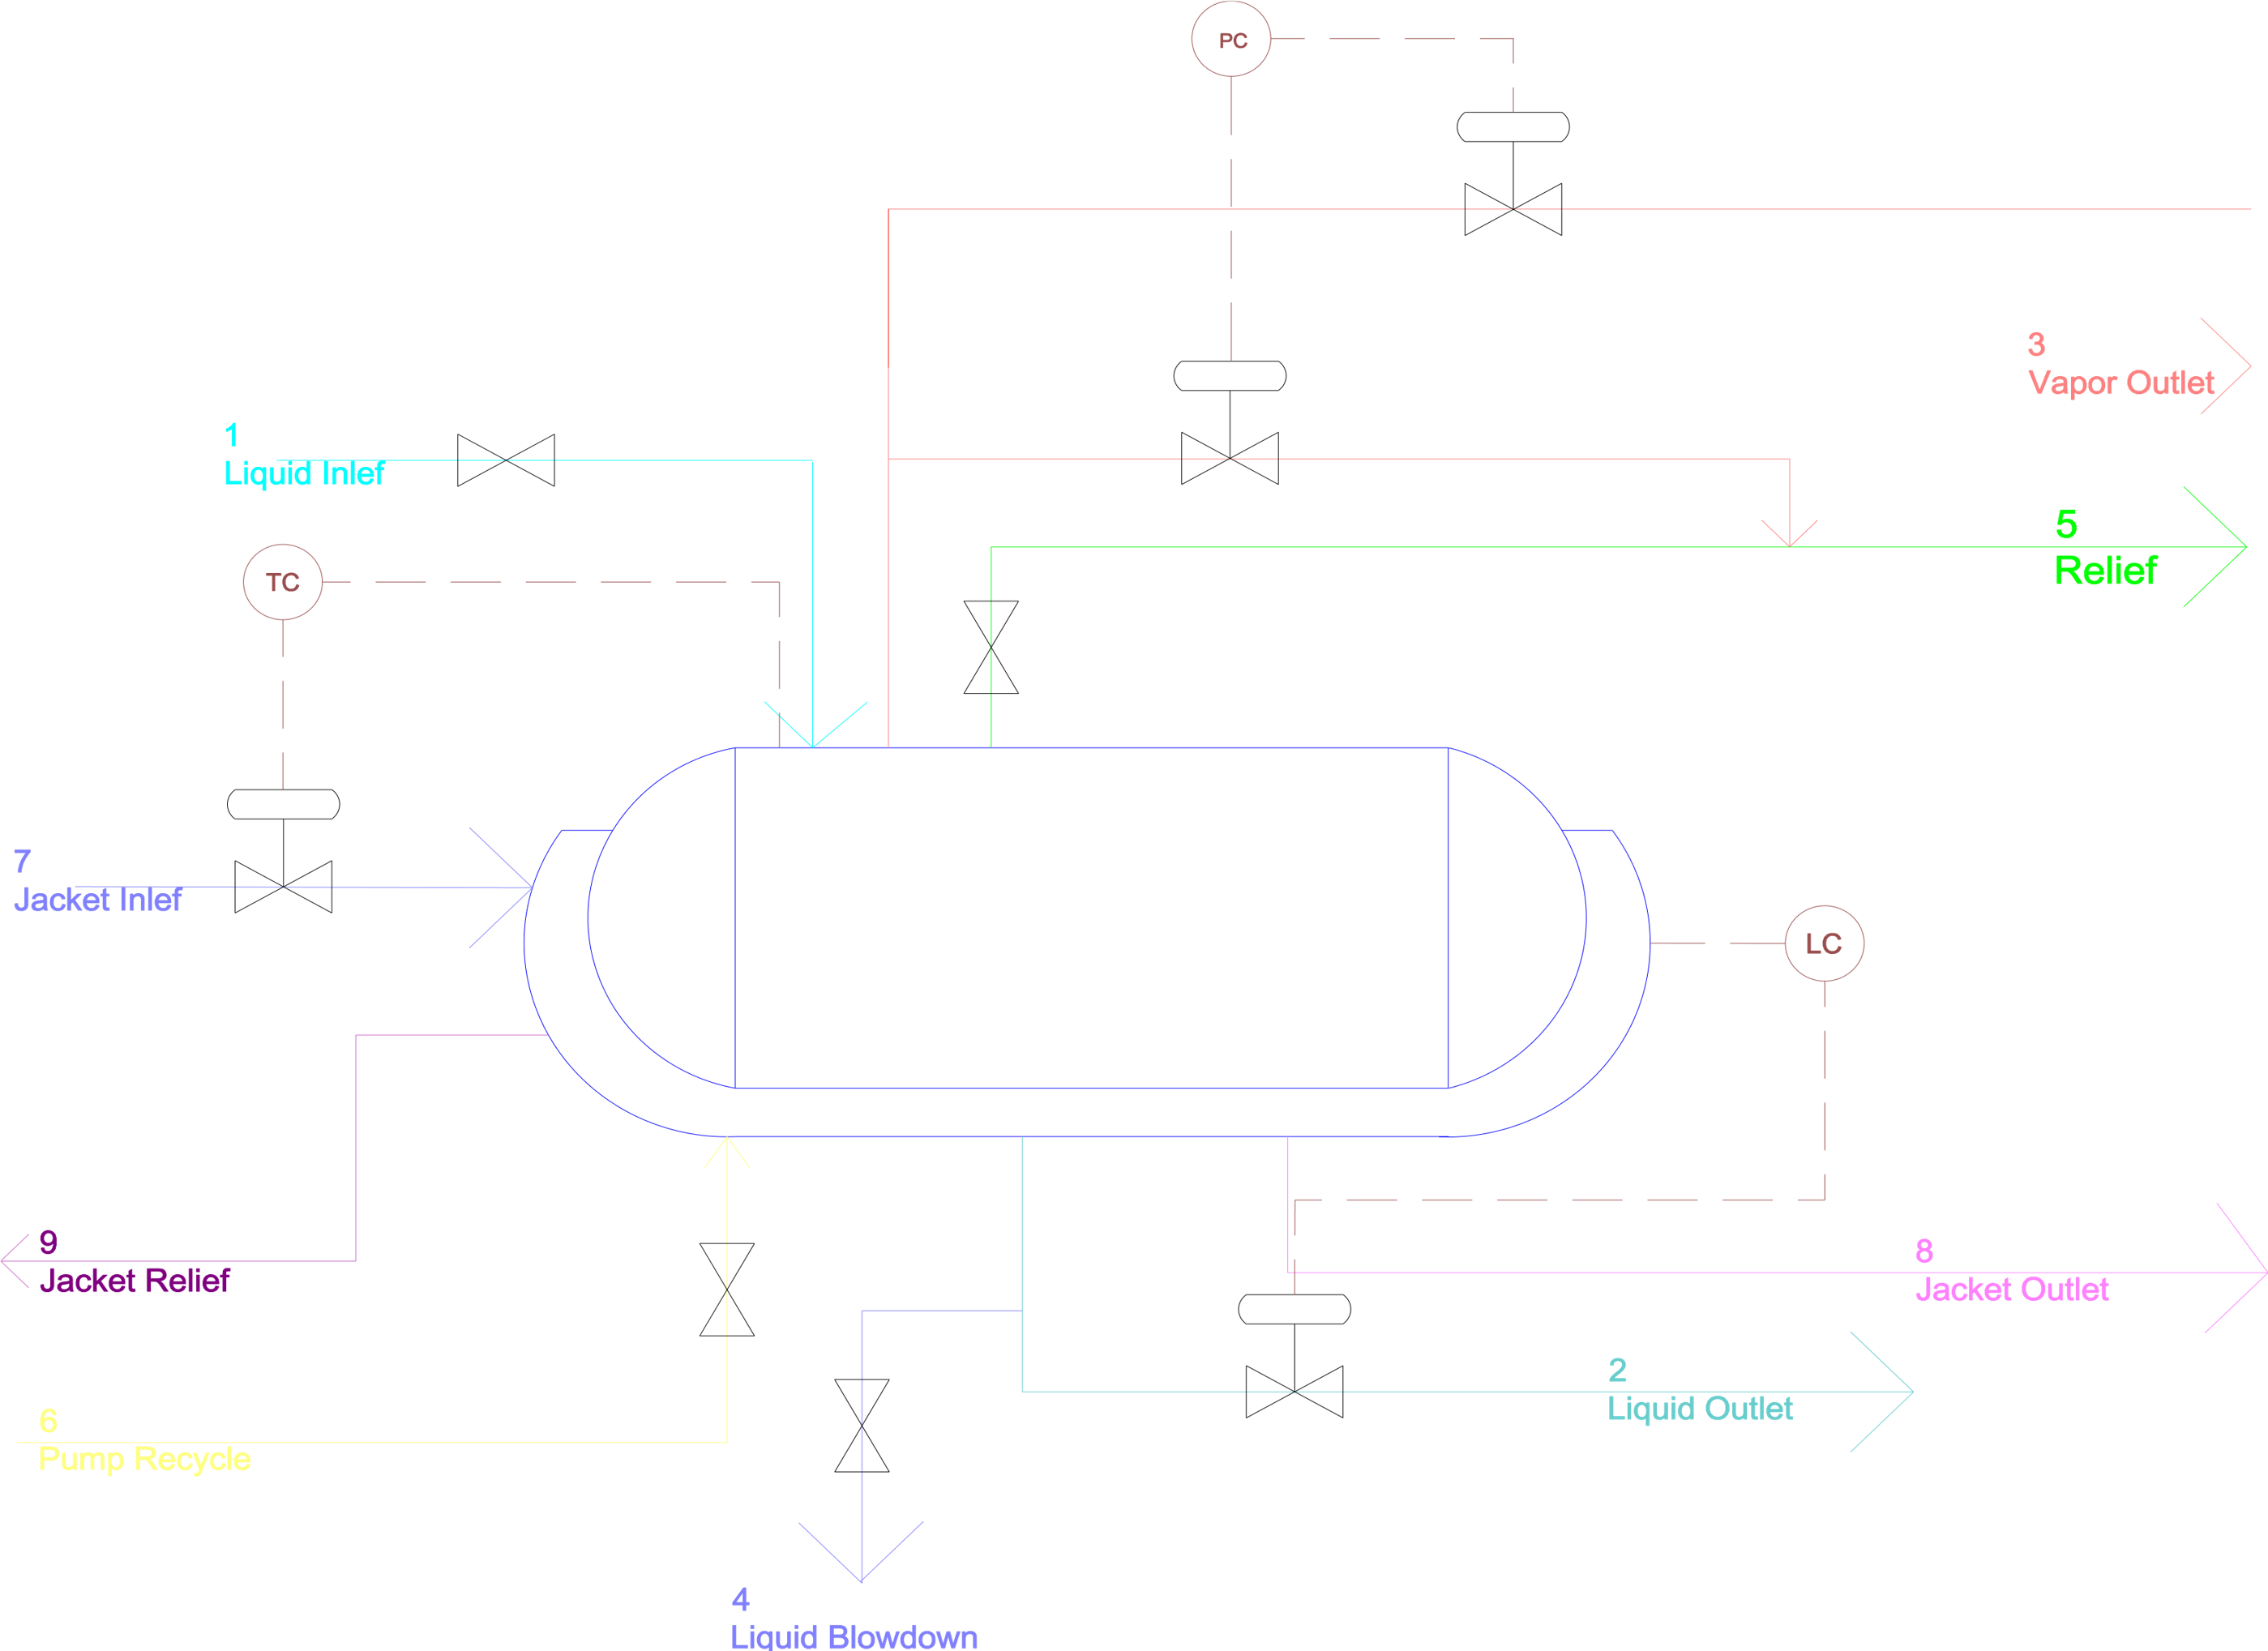
\includegraphics[width=\linewidth]{figuras/pfd.png}
  \caption{Diagrama de Flujo de Procesos — Columna de Absorción con Chaqueta Térmica}
  \label{fig:pfd}
\end{figure}

\subsection{Líneas del proceso}

\renewcommand{\arraystretch}{1.35}
\begin{longtable}{C{1.2cm} L{3.5cm} L{9.5cm}}
\toprule
\rowcolor{ipnguinda}
\color{white}\textbf{No.} & \color{white}\textbf{Corriente} & \color{white}\textbf{Descripción} \\
\midrule
\endfirsthead
\toprule
\rowcolor{ipnguinda}
\color{white}\textbf{No.} & \color{white}\textbf{Corriente} & \color{white}\textbf{Descripción} \\
\midrule
\endhead
\bottomrule
\endfoot
1  & Liquid Inlet     & Alimentación principal al recipiente. Caudal de 80 LPM, DN40, con válvula de aislamiento y medidor electromagnético. \\
\rowcolor{grisclaro}
2  & Liquid Outlet    & Descarga del producto procesado hacia bomba de separación y control de flujo. \\
3  & Vapor Outlet     & Salida de vapor del recipiente. Medición con flujómetro vortex. Caudal 130 LPM, DN25--32. \\
\rowcolor{grisclaro}
4  & Liquid Blowdown  & Purga de condensados y residuos de la parte inferior del tanque. \\
5  & Relief           & Línea de alivio de presión con PSV-3, PIT-6 y PIC-6. \\
\rowcolor{grisclaro}
6  & Pump Recycle     & Retorno de bomba centrífuga Flowserve con VFD. DN25. \\
7  & Jacket Inlet     & Entrada de fluido térmico a la chaqueta, controlada por TCV SAMSON 3241. \\
\rowcolor{grisclaro}
8  & Jacket Outlet    & Retorno del fluido térmico de la chaqueta con medidor electromagnético. \\
9  & Jacket Relief    & Alivio de presión de chaqueta con PSV-2 y válvula Velan API 603. \\
\bottomrule
\end{longtable}

% ============================================================
\section{Diagrama de Tubería e Instrumentación (DTI)}
% ============================================================

El DTI muestra la instrumentación completa del sistema con etiquetas ISA-5.1: transmisores, controladores, elementos primarios, válvulas de control y de aislamiento, así como las señales de proceso.

\begin{figure}[H]
  \centering
  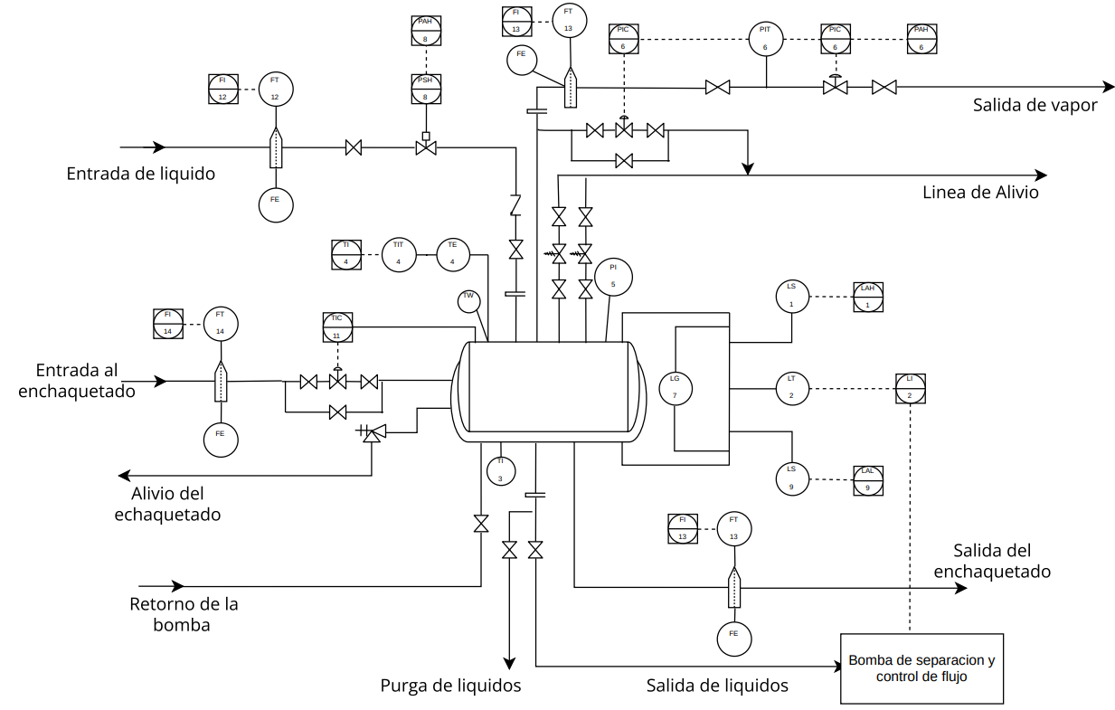
\includegraphics[width=\linewidth]{figuras/dti.png}
  \caption{Diagrama de Tubería e Instrumentación (DTI) — Columna de Absorción}
  \label{fig:dti}
\end{figure}

% ============================================================
\section{Diagrama de Bloques del Sistema}
% ============================================================

La operación del sistema sigue la siguiente secuencia de pasos:

\begin{tcolorbox}[enhanced, colback=grisclaro, colframe=ipnguinda, arc=5pt, boxrule=1pt]
\renewcommand{\arraystretch}{1.4}
\begin{tabular}{C{1.8cm} L{11cm}}
\rowcolor{ipnguinda!15}\textbf{Paso 1} & \textbf{Inspección e Inicio:} Energizar panel de control. Abrir válvulas de aislamiento. \\
\textbf{Paso 2} & \textbf{Carga de Líquido (LIQUID INLET):} Alimentar a 80 LPM. Monitorear LT-2 y LG-7 (Nivel). \\
\rowcolor{ipnguinda!15}\textbf{Paso 3} & \textbf{Recirculación de la Bomba:} Arrancar bomba centrífuga. Ajustar velocidad con VFD. \\
\textbf{Paso 4} & \textbf{Control de Temperatura:} Ajustar TIC a 40°C. Regular válvula TCV en chaqueta. \\
\rowcolor{ipnguinda!15}\textbf{Paso 5} & \textbf{Presurización del Sistema:} Fijar PIC a 2.5 bar manométrica. Regular PCV en salida de vapor. \\
\textbf{Paso 6} & \textbf{Monitoreo y Operación Continua:} Supervisar alarmas (PAH, LAH, LAL). Estado estable. \\
\end{tabular}
\end{tcolorbox}

\subsection{Lista de Componentes del Panel de Control}

\renewcommand{\arraystretch}{1.3}
\begin{longtable}{L{3.2cm} L{4.5cm} L{6.8cm}}
\toprule
\rowcolor{ipnguinda}
\color{white}\textbf{Sistema} & \color{white}\textbf{Instrumentos} & \color{white}\textbf{Justificación} \\
\midrule
\endfirsthead
\toprule
\rowcolor{ipnguinda}
\color{white}\textbf{Sistema} & \color{white}\textbf{Instrumentos} & \color{white}\textbf{Justificación} \\
\midrule
\endhead
\bottomrule
\endfoot
Control de presión       & PI, PIT, PIC, PAH       & Monitorear y controlar presión en tanque, chaqueta y líneas de alivio, asegurando operación segura. \\
\rowcolor{grisclaro}
Control de temperatura   & TE, TI, TIT, TIC         & Control térmico vital para mantener condiciones óptimas en tanque y chaqueta. \\
Control de nivel         & LT, LI, LG, LS, LAL     & Evitar sobrellenado o vaciado garantizando operación continua y segura. \\
\rowcolor{grisclaro}
Control de flujo         & FT (electromagnético y vortex) & Control y monitoreo de caudales críticos en entrada y salida. \\
Control de bomba         & Arranque/parada + VFD   & Ajustar flujo reciclado según demanda, optimizando energía y proceso. \\
\rowcolor{grisclaro}
Alarmas de seguridad     & PAH, LAH, LAL           & Respuesta rápida ante condiciones anómalas, mejorando seguridad. \\
\bottomrule
\end{longtable}

% ============================================================
\section{Lazos de Control (Closed-Loop)}
% ============================================================

El sistema cuenta con tres lazos de control en lazo cerrado que mantienen las variables críticas en su valor de \textit{set point}.

% ---- LAZO NIVEL ----
\subsection{Lazo de Control de Nivel}

\begin{figure}[H]
  \centering
  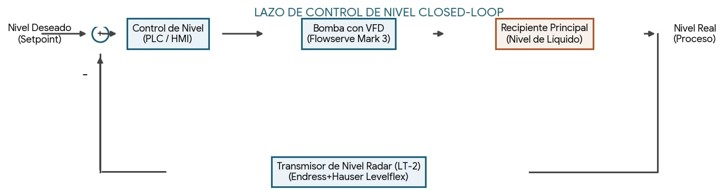
\includegraphics[width=\linewidth]{figuras/lazo_nivel.jpg}
  \caption{Lazo de Control de Nivel — Closed-Loop}
  \label{fig:lazo_nivel}
\end{figure}

\begin{especbox}[title={Parámetros del Lazo de Nivel}]
\renewcommand{\arraystretch}{1.3}
\begin{tabular}{L{4.5cm} L{9cm}}
\textbf{Variable controlada}        & Nivel de líquido en el recipiente principal \\
\textbf{Variable manipulada}        & Velocidad de la bomba centrífuga (VFD) \\
\textbf{Controlador}                & PLC / HMI (Control de Nivel) \\
\textbf{Sensor / Transmisor}        & LT-2 — Endress+Hauser Levelflex FMP54 (radar guiado, \(\pm2\,\)mm) \\
\textbf{Elemento final de control}  & Bomba Flowserve Durco Mark 3 ISO con VFD \\
\textbf{Señal}                      & 4--20\,mA / HART \\
\end{tabular}
\end{especbox}

% ---- LAZO PRESIÓN ----
\subsection{Lazo de Control de Presión}

\begin{figure}[H]
  \centering
  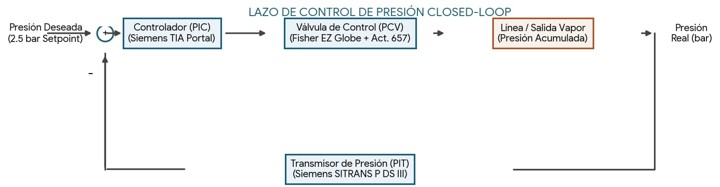
\includegraphics[width=\linewidth]{figuras/lazo_presion.jpg}
  \caption{Lazo de Control de Presión — Closed-Loop}
  \label{fig:lazo_presion}
\end{figure}

\begin{especbox}[title={Parámetros del Lazo de Presión}]
\renewcommand{\arraystretch}{1.3}
\begin{tabular}{L{4.5cm} L{9cm}}
\textbf{Variable controlada}        & Presión acumulada en la línea / salida de vapor \\
\textbf{Set Point}                  & 2.5 bar manométrica \\
\textbf{Controlador}                & PIC — Siemens TIA Portal \\
\textbf{Sensor / Transmisor}        & PIT — Siemens SITRANS P DS III (4--20\,mA, HART) \\
\textbf{Elemento final de control}  & PCV — Fisher EZ Globe Valve + Actuador neumático 657 \\
\textbf{Señal}                      & 4--20\,mA / HART \\
\end{tabular}
\end{especbox}

% ---- LAZO TEMPERATURA ----
\subsection{Lazo de Control de Temperatura}

\begin{figure}[H]
  \centering
  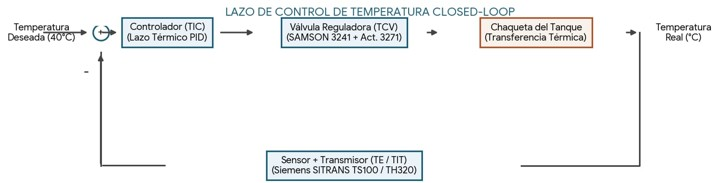
\includegraphics[width=\linewidth]{figuras/lazo_temperatura.jpg}
  \caption{Lazo de Control de Temperatura — Closed-Loop}
  \label{fig:lazo_temp}
\end{figure}

\begin{especbox}[title={Parámetros del Lazo de Temperatura}]
\renewcommand{\arraystretch}{1.3}
\begin{tabular}{L{4.5cm} L{9cm}}
\textbf{Variable controlada}        & Temperatura de la chaqueta del tanque \\
\textbf{Set Point}                  & 40\,°C \\
\textbf{Controlador}                & TIC — Lazo Térmico PID \\
\textbf{Sensor / Transmisor}        & TE — Siemens SITRANS TS100 (PT100) + TIT — TH320 \\
\textbf{Elemento final de control}  & TCV — SAMSON Tipo 3241 + Actuador neumático 3271 \\
\textbf{Señal}                      & 4--20\,mA / HART \\
\end{tabular}
\end{especbox}

% ============================================================
\section{Selección y Especificaciones de Instrumentos}
% ============================================================

% ---- PRESIÓN ----
\subsection{Instrumentos de Presión}

\subsubsection{Transmisor Indicador de Presión (PIT)}

\begin{especbox}[title={PIT — Siemens SITRANS P DS III}]
\renewcommand{\arraystretch}{1.25}
\begin{tabular}{L{4cm} L{9.5cm}}
\textbf{Ubicación}     & Línea de alivio (2 unidades) \\
\textbf{Función}       & Mide presión, transmite señal al sistema de control e indica localmente el valor medido. \\
\textbf{Características} & Mide presión manométrica, absoluta o diferencial. Salida 4--20\,mA HART. Alta precisión. Acero inoxidable 316L. Apto para zonas peligrosas (ATEX). \\
\textbf{Rango}         & 0--2.5 bar manométrica \\
\textbf{Cantidad}      & 2 unidades \\
\end{tabular}
\end{especbox}

\subsubsection{Indicador de Presión (PI)}

\begin{especbox}[title={PI — Manómetro WIKA 232.50}]
\renewcommand{\arraystretch}{1.25}
\begin{tabular}{L{4cm} L{9.5cm}}
\textbf{Ubicación}       & Tanque principal (zona superior) \\
\textbf{Función}         & Mostrar visualmente la presión del proceso de forma analógica, sin acciones de control. \\
\textbf{Características} & Hasta 100\,°C de proceso. Compatible con gases y líquidos industriales. Conexión estándar ½'' NPT. \\
\textbf{Rango}           & 0--2.5 bar manométrica \\
\textbf{Cantidad}        & 1 unidad \\
\end{tabular}
\end{especbox}

\subsubsection{Controlador de Presión (PIC)}

\begin{especbox}[title={PIC — Siemens TIA Portal}]
\renewcommand{\arraystretch}{1.25}
\begin{tabular}{L{4cm} L{9.5cm}}
\textbf{Ubicación}       & Panel de control \\
\textbf{Función}         & Compara la presión medida con el set point y envía señal correctiva a la PCV. \\
\textbf{Características} & Programación de PLCs, redes industriales, diagnóstico en línea y gestión de proyectos. \\
\textbf{Rango}           & 0--2.5 bar manométrica \\
\textbf{Cantidad}        & 3 unidades \\
\end{tabular}
\end{especbox}

\subsubsection{Alarma de Presión Alta (PAH)}

\begin{especbox}[title={PAH — Siemens WinCC}]
\renewcommand{\arraystretch}{1.25}
\begin{tabular}{L{4cm} L{9.5cm}}
\textbf{Ubicación}       & Panel de alarmas integrado \\
\textbf{Función}         & Genera señal de alarma cuando la presión supera el límite preestablecido. \\
\textbf{Características} & Supervisión en tiempo real, gestión de alarmas y eventos, tendencias históricas, generación de reportes. \\
\textbf{Rango}           & Activación a 2.5 bar manométrica \\
\textbf{Cantidad}        & 2 unidades \\
\end{tabular}
\end{especbox}

% ---- TEMPERATURA ----
\subsection{Instrumentos de Temperatura}

\subsubsection{Sensor de Temperatura (TE)}

\begin{especbox}[title={TE — Siemens SITRANS TS100 (PT100)}]
\renewcommand{\arraystretch}{1.25}
\begin{tabular}{L{4cm} L{9.5cm}}
\textbf{Ubicación}       & Dentro del thermowell TW10 en el tanque \\
\textbf{Función}         & Elemento primario que detecta la temperatura y la convierte en señal eléctrica medible. \\
\textbf{Características} & Configuración 3 hilos (industrial). Rango --50 a 250\,°C. Acero inoxidable 316L. Apto para zonas explosivas. \\
\textbf{Rango operación} & 40\,°C \\
\textbf{Cantidad}        & 1 unidad \\
\end{tabular}
\end{especbox}

\subsubsection{Thermowell (TW)}

\begin{especbox}[title={TW — WIKA TW10}]
\renewcommand{\arraystretch}{1.25}
\begin{tabular}{L{4cm} L{9.5cm}}
\textbf{Ubicación}       & Tanque principal \\
\textbf{Función}         & Alojar y proteger el sensor de temperatura del contacto directo con el fluido. Permite retirar el sensor sin detener la operación. \\
\textbf{Características} & Acero inoxidable 316. Conexiones ½'' NPT. Longitud de inserción 100--200\,mm. Resistente a presión y flujo interno. \\
\textbf{Rango operación} & 40\,°C \\
\textbf{Cantidad}        & 1 unidad \\
\end{tabular}
\end{especbox}

\subsubsection{Transmisor Indicador de Temperatura (TIT)}

\begin{especbox}[title={TIT — Siemens SITRANS TH320}]
\renewcommand{\arraystretch}{1.25}
\begin{tabular}{L{4cm} L{9.5cm}}
\textbf{Ubicación}       & Entrada y salida de la chaqueta \\
\textbf{Función}         & Mide la temperatura, transmite señal estandarizada al PLC y presenta la lectura localmente. \\
\textbf{Características} & Rango 4--20\,mA. Convierte señal TS100. Montaje cabeza tipo DIN. Configuración HART. \\
\textbf{Rango operación} & 40\,°C \\
\textbf{Cantidad}        & 1 unidad \\
\end{tabular}
\end{especbox}

\subsubsection{Indicador de Temperatura (TI)}

\begin{especbox}[title={TI — WIKA A53 Bimetálico Industrial}]
\renewcommand{\arraystretch}{1.25}
\begin{tabular}{L{4cm} L{9.5cm}}
\textbf{Ubicación}       & Tanque principal \\
\textbf{Función}         & Mostrar localmente la temperatura medida en el proceso industrial. \\
\textbf{Características} & Carcasa acero inoxidable 316. Montaje inferior. Compatibilidad con solventes de hidrocarburos. \\
\textbf{Rango operación} & 40\,°C \\
\textbf{Cantidad}        & 2 unidades \\
\end{tabular}
\end{especbox}

% ---- NIVEL ----
\subsection{Instrumentos de Nivel}

\subsubsection{Transmisor de Nivel (LT-2)}

\begin{especbox}[title={LT-2 — Endress+Hauser Levelflex FMP54}]
\renewcommand{\arraystretch}{1.25}
\begin{tabular}{L{4cm} L{9.5cm}}
\textbf{Ubicación}       & Parte superior lateral del recipiente principal \\
\textbf{Función}         & Medir continuamente el nivel del líquido y enviar señal al sistema de control. \\
\textbf{Características} & Rango hasta 45\,m. Precisión ±2\,mm. Acero inoxidable 316L. Salida 4--20\,mA/HART. IP66/IP68. \\
\textbf{Principio}       & Radar de onda guiada (TDR). No depende de densidad ni conductividad del fluido. \\
\textbf{Cantidad}        & 1 unidad \\
\end{tabular}
\end{especbox}

\subsubsection{Indicador de Nivel (LI-2)}

\begin{especbox}[title={LI-2 — Siemens SITRANS RD100}]
\renewcommand{\arraystretch}{1.25}
\begin{tabular}{L{4cm} L{9.5cm}}
\textbf{Ubicación}       & Panel local o tablero cercano al recipiente \\
\textbf{Función}         & Mostrar continuamente el nivel medido por LT-2 para monitoreo operacional. \\
\textbf{Características} & Configurable 4--20\,mA. Precisión ±0.1\%. Pantalla LCD digital. IP65. \\
\textbf{Cantidad}        & 1 unidad \\
\end{tabular}
\end{especbox}

\subsubsection{Indicador Visual de Nivel (LG-7)}

\begin{especbox}[title={LG-7 — Kobold BNA Magnetic Level Indicator}]
\renewcommand{\arraystretch}{1.25}
\begin{tabular}{L{4cm} L{9.5cm}}
\textbf{Ubicación}       & Costado externo del tanque (bypass) \\
\textbf{Función}         & Permitir visualización directa del nivel real sin contacto con el fluido. \\
\textbf{Características} & Flotador magnético bicolor. Acero inoxidable 316. Precisión ±10\,mm. IP65. Opera sin energía eléctrica. \\
\textbf{Cantidad}        & 1 unidad \\
\end{tabular}
\end{especbox}

\subsubsection{Interruptores de Nivel (LS-1 / LS-9)}

\begin{especbox}[title={LS-1/LS-9 — VEGA VEGASWING 63}]
\renewcommand{\arraystretch}{1.25}
\begin{tabular}{L{4cm} L{9.5cm}}
\textbf{LS-1 ubicación}  & Nivel alto del recipiente (80--90\% del rango) \\
\textbf{LS-9 ubicación}  & Nivel bajo del recipiente (10--20\% del rango) \\
\textbf{Función}         & Detectar niveles críticos y activar alarmas o acciones ON/OFF. \\
\textbf{Características} & Principio vibratorio (horquilla). Acero inoxidable 316L. Salida relé. IP66/IP68. Respuesta $\leq$1\,s. \\
\textbf{Cantidad}        & 2 unidades \\
\end{tabular}
\end{especbox}

\subsubsection{Alarmas de Nivel (LAH-1 / LAL-9)}

\begin{especbox}[title={LAH-1 / LAL-9 — Patlite LR6 Signal Tower}]
\renewcommand{\arraystretch}{1.25}
\begin{tabular}{L{4cm} L{9.5cm}}
\textbf{Ubicación}       & Panel de control o estructura visible \\
\textbf{LAH-1 función}   & Alertar condición de sobrellenado. Activada por LS-1. Señal roja. \\
\textbf{LAL-9 función}   & Alertar nivel mínimo o vaciado excesivo. Activada por LS-9. Señal amarilla/ámbar. \\
\textbf{Características} & Alarma luminosa y sonora. 85--90\,dB @ 1\,m. Policarbonato industrial. IP65. \\
\textbf{Cantidad}        & 2 unidades \\
\end{tabular}
\end{especbox}

% ---- FLUJO ----
\subsection{Instrumentos de Flujo}

\begin{notabox}
\textbf{Criterio de selección:} Se emplean medidores electromagnéticos para todas las líneas de líquido (agua + solventes, conductividad $>5\,\mu$S/cm) y medidor vortex para la línea de vapor (baja densidad, 0.0017\,g/cm³, no conductor).
\end{notabox}

\subsubsection{Medidor Electromagnético — Endress+Hauser Promag P 300}

\begin{especbox}[title={FT (Líquidos) — E+H Promag P 300}]
\renewcommand{\arraystretch}{1.25}
\begin{tabular}{L{4.5cm} L{9cm}}
\textbf{Líneas aplicadas}   & Liquid Inlet, Jacket Inlet, Jacket Outlet, Liquid Outlet, Pump Recycle \\
\textbf{Precisión}          & ±0.5\% del valor medido ± 1\,mm/s \\
\textbf{Rango de flujo}     & 4\,dm³/min a 9\,600\,m³/h \\
\textbf{DN recomendado}     & DN40 (1½'') para 80\,LPM; DN25 para Pump Recycle \\
\textbf{Temperatura máx.}   & 150\,°C \\
\textbf{Presión máx.}       & PN40 / Clase 300 \\
\textbf{Material electrodo} & Hastelloy C o Titanio (resistencia a solventes) \\
\textbf{Revestimiento}      & PFA / PTFE \\
\textbf{Salida}             & 4--20\,mA + HART / PROFIBUS \\
\textbf{Certificación}      & ATEX/IECEx Zona 1 \\
\end{tabular}
\end{especbox}

\subsubsection{Medidor Vortex — Endress+Hauser Prowirl F 200}

\begin{especbox}[title={FT (Vapor) — E+H Prowirl F 200}]
\renewcommand{\arraystretch}{1.25}
\begin{tabular}{L{4.5cm} L{9cm}}
\textbf{Línea aplicada}   & Vapor Outlet \\
\textbf{Precisión}        & ±1.0\% del valor medido \\
\textbf{Rango de flujo}   & 0.39 a 28\,000\,m³/h \\
\textbf{DN recomendado}   & DN25--32 (1--1¼'') para 130\,LPM de vapor \\
\textbf{Temperatura máx.} & 260\,°C (estándar) \\
\textbf{Presión máx.}     & 0--10\,bar \\
\textbf{Material cuerpo}  & Acero inoxidable 316L \\
\textbf{Salida}           & 4--20\,mA + HART \\
\textbf{Tramos rectos}    & 10D aguas arriba, 5D aguas abajo \\
\end{tabular}
\end{especbox}

\subsection{Diámetros Nominales de Tuberías}

\renewcommand{\arraystretch}{1.3}
\begin{tabular}{L{4cm} C{2.5cm} C{2.5cm} L{4.5cm}}
\toprule
\rowcolor{ipnguinda}
\color{white}\textbf{Línea} & \color{white}\textbf{Caudal} & \color{white}\textbf{DN} & \color{white}\textbf{Instrumento} \\
\midrule
Liquid Inlet   & 80 LPM       & DN40 (1½'') & Electromagnético \\
\rowcolor{grisclaro}
Jacket Inlet/Outlet & Variable & DN25--40    & Electromagnético \\
Liquid Outlet  & 80 LPM       & DN40 (1½'') & Electromagnético \\
\rowcolor{grisclaro}
Vapor Outlet   & 130 LPM      & DN25--32    & Vortex \\
Pump Recycle   & $<$80 LPM    & DN25 (1'')  & Electromagnético \\
\bottomrule
\end{tabular}

% ============================================================
\section{Válvulas del Sistema}
% ============================================================

\subsection{Válvula de Control de Presión (PCV)}

\begin{especbox}[title={PCV — Fisher EZ Globe Valve + Actuador 657}]
\renewcommand{\arraystretch}{1.25}
\begin{tabular}{L{4cm} L{9.5cm}}
\textbf{Ubicación}       & Línea de vapor de entrada a la chaqueta \\
\textbf{Función}         & Controlar la presión del vapor que ingresa a la chaqueta para mantener presión de operación estable. \\
\textbf{Material}        & SS316 \\
\textbf{Actuador}        & Neumático diafragma-resorte. Señal 4--20\,mA. \\
\textbf{Acción de falla} & Falla cerrada (FC) — corta vapor ante pérdida de señal o aire. \\
\textbf{Norma}           & ANSI 150, ISA 75.01 \\
\textbf{Rango}           & 0--10\,bar, DN25--32 \\
\end{tabular}
\end{especbox}

\subsection{Válvula de Control de Temperatura (TCV)}

\begin{especbox}[title={TCV — SAMSON Tipo 3241 + Actuador 3271}]
\renewcommand{\arraystretch}{1.25}
\begin{tabular}{L{4cm} L{9.5cm}}
\textbf{Ubicación}       & Entrada del fluido de calentamiento/enfriamiento de la chaqueta \\
\textbf{Función}         & Regular caudal del fluido térmico para mantener temperatura del tanque en el set point. \\
\textbf{Material}        & SS316 y SS316L \\
\textbf{Actuador}        & Neumático. Señal 4--20\,mA. \\
\textbf{Acción de falla} & Falla cerrada (FC) \\
\textbf{Norma}           & ANSI 150, IEC 60534 \\
\textbf{Rango}           & -50 a 220\,°C, DN25--32 \\
\end{tabular}
\end{especbox}

\subsection{Válvulas de Alivio (PSV-1, PSV-2, PSV-3)}

\begin{especbox}[title={PSV — Elevación Completa con Resorte, API 520}]
\renewcommand{\arraystretch}{1.25}
\begin{tabular}{L{4cm} L{9.5cm}}
\textbf{PSV-1 ubicación} & Tanque principal \\
\textbf{PSV-2 ubicación} & Chaqueta \\
\textbf{PSV-3 ubicación} & Línea de alivio \\
\textbf{Función}         & Alivio de sobrepresión por apertura automática al superar la presión de ajuste. \\
\textbf{Material}        & WCB (acero al carbono) + SS304 (disco, asiento, guía) \\
\textbf{Rango}           & 10 a 400\,PSIG (0.7 a 27.6\,bar) \\
\textbf{Cantidad}        & 3 unidades \\
\end{tabular}
\end{especbox}

\subsection{Válvulas de Aislamiento}

\renewcommand{\arraystretch}{1.3}
\begin{longtable}{L{3cm} L{3.5cm} L{3.5cm} L{4.5cm}}
\toprule
\rowcolor{ipnguinda}
\color{white}\textbf{Línea} & \color{white}\textbf{Modelo} & \color{white}\textbf{Tipo} & \color{white}\textbf{Rango} \\
\midrule
\endfirsthead
\toprule
\rowcolor{ipnguinda}
\color{white}\textbf{Línea} & \color{white}\textbf{Modelo} & \color{white}\textbf{Tipo} & \color{white}\textbf{Rango} \\
\midrule
\endhead
\bottomrule
\endfoot
Liquid Inlet/Outlet  & Flow-Tek S19 SS316 & Bola flotante Full Port, RPTFE & DN25--50, Clase 150, hasta 20\,bar \\
\rowcolor{grisclaro}
Jacket Inlet/Outlet  & KITZ Serie U SS316 & Full Bore, PTFE & ANSI 150, DN25--50 \\
Vapor Outlet, Jacket Relief & Velan API 603 SS316 & Apertura total & ANSI 150, DN15--600 \\
\rowcolor{grisclaro}
Pump Recycle         & Worcester Serie 59 & Alta frecuencia & ANSI 150, DN25--50 \\
\bottomrule
\end{longtable}

\subsection{Bomba de Reciclaje}

\begin{especbox}[title={Bomba Centrífuga — Flowserve Durco Mark 3 ISO + VFD}]
\renewcommand{\arraystretch}{1.25}
\begin{tabular}{L{4cm} L{9.5cm}}
\textbf{Ubicación}      & Línea Pump Recycle \\
\textbf{Función}        & Recirculación del fluido de proceso con ajuste eficiente de caudal mediante VFD. \\
\textbf{Caudal máx.}   & 475\,m³/h (2091\,gpm) \\
\textbf{Altura máx.}   & 150\,m \\
\textbf{Presión máx.}  & 25\,bar \\
\textbf{Temperatura}   & --40\,°C a 300\,°C \\
\textbf{Material}       & Acero inoxidable 316L \\
\textbf{Sello}          & Mecánico doble API 682 (solventes inflamables) \\
\textbf{Norma}          & API 610, ASME B73.1 \\
\end{tabular}
\end{especbox}

% ============================================================
\section{Instalación Típica de Instrumentos}
% ============================================================

\subsection{Instrumentos de Presión}

\textbf{Indicador de Presión (PI) — WIKA 232.50}
\begin{enumerate}[leftmargin=1.5cm, label=\arabic*.]
  \item Conexión al proceso mediante toma roscada ½'' NPT soldada a la boquilla del tanque.
  \item Instalar sello de diafragma entre toma y manómetro (protección frente a solventes).
  \item Válvula de bola ½'' para aislamiento y mantenimiento.
  \item Sifón pigtail de acero inoxidable 316 (protección contra altas temperaturas).
  \item Montaje vertical con carátula hacia el operador, a la misma altura del punto de toma.
\end{enumerate}

\textbf{Transmisor PIT — Siemens SITRANS P DS III}
\begin{enumerate}[leftmargin=1.5cm, label=\arabic*.]
  \item Toma de presión ½'' NPT en lateral/superior de la tubería de alivio.
  \item Manifold de 3 válvulas (bloqueo, venteo, ecualización) — permite calibración en línea.
  \item Tubing de acero inoxidable 316 OD ½'' con pendiente descendente mínima de 1:12.
  \item Montaje en soporte tipo L/U. Orientación con diafragma hacia abajo (autodrenaje).
  \item Cable HART apantallado 2 hilos, prensaestopas ATEX. Pantalla a tierra en el tablero.
\end{enumerate}

\textbf{Válvula PCV — Fisher EZ + Actuador 657}
\begin{enumerate}[leftmargin=1.5cm, label=\arabic*.]
  \item Tramo recto mínimo 10D aguas arriba y 5D aguas abajo.
  \item Válvulas de compuerta de aislamiento + bypass manual con válvula globo.
  \item Aire de instrumento seco y filtrado (1.4--6\,bar) vía tubing ¼'' OD.
  \item Posicionador Fisher DVC6200 montado sobre actuador. Señal 4--20\,mA del PLC.
  \item Filtro-regulador de aire (AFR) aguas arriba del actuador.
  \item Configuración: falla cerrada (FC). Montaje horizontal con actuador hacia arriba.
\end{enumerate}

\subsection{Instrumentos de Temperatura}

\textbf{Thermowell (TW) — WIKA TW10}
\begin{enumerate}[leftmargin=1.5cm, label=\arabic*.]
  \item Conexión ½'' NPT soldada a boquilla del tanque (cumpliendo ASME B31.3).
  \item Longitud de inmersión mínima 100\,mm (típica 150--200\,mm).
  \item Orientación horizontal o 15° respecto a la horizontal, punta apuntando aguas abajo del flujo.
  \item Verificación de frecuencia natural $\geq2.5\times$ la de desprendimiento de vórtices (ASME PTC 19.3).
  \item Prueba hidrostática a $1.5\times$MAWP antes de instalar el sensor.
\end{enumerate}

\textbf{Sensor PT100 (TE) — Siemens SITRANS TS100}
\begin{enumerate}[leftmargin=1.5cm, label=\arabic*.]
  \item Insertar el PT100 hasta que la punta haga contacto con el fondo del thermowell.
  \item Aplicar pasta conductora térmica en la punta.
  \item Asegurar con cabeza de conexión DIN roscada al thermowell.
  \item Conectar en configuración 3 hilos (compensación de resistencia de cable).
  \item Si el transmisor es remoto, tendido de cable apantallado de 3 hilos (máx. 30\,m).
\end{enumerate}

\subsection{Instrumentos de Nivel}

\textbf{Transmisor Radar Guiado (LT-2) — E+H Levelflex FMP54}
\begin{enumerate}[leftmargin=1.5cm, label=\arabic*.]
  \item Boquilla dedicada en parte superior del tanque (DN50 mínimo, bridada preferida).
  \item Sonda guiada vertical, desde parte superior hasta 50\,mm sobre el fondo (sin tocar).
  \item Distancia mínima de 200\,mm entre sonda y paredes o estructuras internas.
  \item Respeto de zona muerta superior (50--100\,mm desde la brida).
  \item Mapeo de eco falso con tanque vacío antes de la puesta en marcha.
\end{enumerate}

\textbf{Indicador Magnético (LG-7) — Kobold BNA}
\begin{enumerate}[leftmargin=1.5cm, label=\arabic*.]
  \item Conexiones superior e inferior al tanque mediante bridas.
  \item Válvulas de bola en ambas conexiones (aislamiento sin vaciar tanque).
  \item Válvula de drenaje ¼'' en la parte inferior del cuerpo.
  \item Verticalidad ±1° (verificar con nivel de burbuja).
  \item Centro de escala a 1.2--1.6\,m sobre plataforma del operador.
\end{enumerate}

\textbf{Interruptores de Nivel (LS-1/LS-9) — VEGA VEGASWING 63}
\begin{enumerate}[leftmargin=1.5cm, label=\arabic*.]
  \item Montaje lateral con conexión roscada ¾'' o 1'' NPT en puntos de nivel crítico.
  \item LS-1 en nivel alto (80--90\%); LS-9 en nivel bajo (10--20\%).
  \item Horquilla vibratoria orientada horizontalmente hacia el interior del tanque.
  \item Conexión 2 hilos a salida de relé, conectada al PLC para LAH-1 y LAL-9.
\end{enumerate}

\subsection{Instrumentos de Flujo}

\textbf{Medidor Electromagnético — E+H Promag P 300}
\begin{enumerate}[leftmargin=1.5cm, label=\arabic*.]
  \item Tramo recto: mínimo 5D aguas arriba y 2D aguas abajo (10D si hay válvula de control antes).
  \item En tubería horizontal: electrodos en posición 3 y 9 horas (evitar burbujas).
  \item En tubería vertical: flujo ascendente (garantiza tubo lleno).
  \item Anillos de tierra (grounding rings) obligatorios en tuberías con revestimiento.
  \item No instalar en punto más alto de la tubería ni inmediatamente después de una bomba.
\end{enumerate}

\textbf{Medidor Vortex — E+H Prowirl F 200}
\begin{enumerate}[leftmargin=1.5cm, label=\arabic*.]
  \item Tramo recto: mínimo 10D aguas arriba y 5D aguas abajo.
  \item Instalación horizontal con transmisor hacia arriba (evitar condensado en sensor).
  \item No aislar el cuerpo del transmisor electrónico.
  \item Válvulas de compuerta (no de bola) aguas arriba y abajo.
  \item Punto de drenaje aguas abajo para purga de condensado.
\end{enumerate}

% ============================================================
\section{Puesta en Operación y Calibración}
% ============================================================

\subsection{Fase 1 — Verificación Pre-Operativa (Pre-Commissioning)}

\renewcommand{\arraystretch}{1.3}
\begin{longtable}{C{0.8cm} L{5.5cm} L{8cm}}
\toprule
\rowcolor{ipnguinda}
\color{white}\textbf{No.} & \color{white}\textbf{Actividad} & \color{white}\textbf{Criterio de Aceptación} \\
\midrule
\endfirsthead
\toprule
\rowcolor{ipnguinda}
\color{white}\textbf{No.} & \color{white}\textbf{Actividad} & \color{white}\textbf{Criterio de Aceptación} \\
\midrule
\endhead
\bottomrule
\endfoot
1 & Inspección visual de montaje         & Todos los instrumentos instalados según especificaciones, sin daños visibles \\
\rowcolor{grisclaro}
2 & Verificación de conexiones de proceso & Tomas, boquillas y válvulas correctamente apretadas y selladas \\
3 & Verificación de cableado eléctrico   & Continuidad, aislamiento $\geq100\,$M$\Omega$ (megger a 500\,VDC), polaridad correcta \\
\rowcolor{grisclaro}
4 & Verificación de aire de instrumento  & Presión 5--7\,bar, seco (punto de rocío $<$-40\,°C), libre de aceite \\
5 & Verificación de puesta a tierra      & Resistencia de tierra $<10\,\Omega$ por instrumento \\
\rowcolor{grisclaro}
6 & Clasificación de área                & Instrumentos en zonas clasificadas con certificación ATEX/IECEx \\
7 & Revisión de documentación            & Hojas de datos, loop diagrams y procedimientos de calibración disponibles \\
\rowcolor{grisclaro}
8 & Prueba hidrostática de tuberías      & Todas las líneas probadas a $1.5\times$ presión de diseño, sin fugas \\
\bottomrule
\end{longtable}

\subsection{Fase 2 — Verificación de Lazos (Loop Check)}

\begin{enumerate}[leftmargin=1.5cm, label=\arabic*.]
  \item Inyectar señal simulada en el transmisor (calibrador de lazo) y verificar lectura en indicador local, HMI/SCADA (WinCC) y registro del PLC.
  \item Simular condiciones de alarma y verificar activación de PAH, LAH y LAL.
  \item Desde el PLC, enviar 4--20\,mA a PCV y TCV y verificar recorrido completo (0 a 100\%).
  \item Documentar resultados en formato de verificación de lazos.
\end{enumerate}

\subsection{Fase 3 — Puesta en Marcha Inicial (Commissioning)}

\begin{enumerate}[leftmargin=1.5cm, label=\arabic*.]
  \item \textbf{Llenado inicial:} Llenar tanque gradualmente monitoreando LT-2, LG-7, LS-1, LS-9 y LI-2.
  \item \textbf{Arranque de bomba:} Arrancar a velocidad mínima (VFD 20--30\%). Verificar dirección de rotación, vibración ($<4.5\,$mm/s RMS per ISO 10816), presión de descarga y caudal.
  \item \textbf{Circulación por chaqueta:} Abrir gradualmente TCV y verificar circulación. Monitorear TIT en entrada y salida.
  \item \textbf{Estabilización:} Operar mínimo 4\,h verificando estabilidad de P, T, L y F.
  \item \textbf{Alarmas en vivo:} Llevar nivel hasta puntos de alarma para verificar LS-1, LS-9, LAH-1 y LAL-9.
  \item \textbf{Sintonización PID:} Método de respuesta escalón o autotuning del PLC para PIC y TIC.
\end{enumerate}

\subsection{Calibración de Instrumentos de Presión}

\textbf{PI — WIKA 232.50:} Calibrador de peso muerto o digital (Fluke 700G). Aplicar presión en 5 puntos (0, 25, 50, 75, 100\% del span), ascenso y descenso. \textbf{Criterio:} Error $\leq\pm1.6\%$ del span (clase 1.6 ASME B40.100). Frecuencia: 12 meses.

\textbf{PIT — SITRANS P DS III:} Calibrador de presión (exactitud $\geq4\times$ la del transmisor) + calibrador de lazo 4--20\,mA. 5 puntos. \textbf{Criterio:} Error $\leq\pm0.15\%$ del span. 4\,mA $=$ 0\%, 20\,mA $=$ 100\%. Frecuencia: 12 meses; verificación de cero trimestral.

\textbf{PSV — API 520:} Banco de prueba certificado. Prueba de pop (presión de apertura), hermeticidad a 90\% del set point y reseat ($\geq93\%$ del set point, blowdown $\leq7\%$). Frecuencia: 12 meses per API 576.

\subsection{Calibración de Instrumentos de Temperatura}

\textbf{PT100 (TE) — SITRANS TS100:} Baño seco + termómetro de referencia certificado. 5 puntos: 0, 10, 20, 30, 40\,°C. Medir resistencia con ohmímetro de precisión 4 hilos. \textbf{Criterio Clase A:} $\pm(0.15+0.002\times|T|)\,°C$. A 40\,°C: $\pm0.23\,°C$. Si falla, reemplazar (no se ajusta). Frecuencia: 24 meses.

\textbf{TIT — SITRANS TH320:} Simulador de resistencia (decade resistance box). Simular 5 valores RTD (100.00 a 115.54\,$\Omega$). \textbf{Criterio:} Error $\leq\pm0.1\,°C$. Ajuste via HART si necesario. Frecuencia: 12 meses.

\textbf{TI — WIKA A53:} Baño de calibración. 3 puntos mínimo (0, 20, 40\,°C). \textbf{Criterio:} Error $\leq\pm1\%$ del span. Frecuencia: 12 meses.

\subsection{Calibración de Instrumentos de Nivel}

\textbf{LT-2 — Levelflex FMP54:} Calibración húmeda in-situ. Con tanque vacío: distancia de referencia 0\%. Con tanque lleno: distancia 100\%. Verificar linealidad a 25, 50 y 75\%. \textbf{Criterio:} Error $\leq\pm2\,$mm. Ejecutar mapeo de eco falso con tanque vacío. Frecuencia: 24 meses.

\textbf{LG-7 — Kobold BNA:} Verificación visual. Llenar tanque a nivel conocido y comparar con LT-2. \textbf{Criterio:} Error $\leq\pm10\,$mm. Frecuencia: 12 meses.

\textbf{LS-1/LS-9 — VEGASWING 63:} Verificación funcional. Llenar/vaciar hasta punto de disparo y verificar conmutación del relé con multímetro. \textbf{Criterio:} Conmutación correcta, tiempo de respuesta $\leq1\,$s. Frecuencia: 6 meses (instrumentos de seguridad, per IEC 61511).

\subsection{Calibración de Instrumentos de Flujo}

\textbf{Promag P 300:} Verificación de cero con flujo detenido (lectura 0.0\,LPM y salida 4.00\,mA). Verificar integridad de electrodos e impedancia mediante diagnóstico del transmisor. \textbf{Criterio:} Error $\leq\pm0.5\%$ + 1\,mm/s. Frecuencia: verificación de cero cada 6 meses; calibración banco de flujo cada 5 años.

\textbf{Prowirl F 200:} Verificar K-factor grabado en fábrica contra certificado de calibración. Verificar sensores de PT y TT integrados. \textbf{Criterio:} Error $\leq\pm1\%$. Frecuencia: 24 meses.

\subsection{Calibración de Válvulas de Control}

\textbf{PCV y TCV:} Calibrador de lazo 4--20\,mA + regulador de presión de aire.
\begin{itemize}
  \item \textbf{Prueba de recorrido:} 4\,mA$\to$0\%, 8\,mA$\to$25\%, 12\,mA$\to$50\%, 16\,mA$\to$75\%, 20\,mA$\to$100\%. Error $\leq\pm1\%$ por punto.
  \item \textbf{Tiempo de respuesta:} 10\% a 90\% del recorrido en 2--10\,s.
  \item \textbf{Hermeticidad de asiento:} Clase IV $\leq0.01\%\,C_v$; Clase V $\leq5\times10^{-4}$\,mL/min/pulgada.
  \item \textbf{Calibración del posicionador:} DVC6200 (Fisher) / SAMSON 3730 para 4--20\,mA $=$ 0--100\%.
  \item \textbf{Prueba parcial de recorrido} (partial stroke test) cada 3 meses.
\end{itemize}
Frecuencia: 12 meses.

% ============================================================
\section{Bibliografía y Normas de Referencia}
% ============================================================

\begin{enumerate}[leftmargin=1.5cm, label={[\arabic*]}]
  \item ISA-5.1 — \textit{Instrumentation Symbols and Identification}. International Society of Automation.
  \item API 520/521 — \textit{Sizing, Selection, and Installation of Pressure-Relieving Devices}. American Petroleum Institute.
  \item ASME B31.3 — \textit{Process Piping}. American Society of Mechanical Engineers.
  \item IEC 60751 — \textit{Industrial Platinum Resistance Thermometers and Platinum Temperature Sensors}.
  \item IEC 60534 — \textit{Industrial-Process Control Valves}.
  \item ASME PTC 19.3 — \textit{Thermowells — Performance Test Codes}.
  \item API 610 — \textit{Centrifugal Pumps for Petroleum, Petrochemical and Natural Gas Industries}.
  \item API 682 — \textit{Pumps — Shaft Sealing Systems for Centrifugal and Rotary Pumps}.
  \item ISO 10816 — \textit{Mechanical Vibration — Evaluation of Machine Vibration by Measurements on Non-Rotating Parts}.
  \item IEC 61511 — \textit{Functional Safety — Safety Instrumented Systems for the Process Industry Sector}.
  \item ANSI/FCI 70-2 — \textit{Control Valve Seat Leakage}. Fluid Controls Institute.
  \item AGA Report No. 7 — \textit{Measurement of Gas by Turbine Meters}. American Gas Association.
  \item Siemens AG — \textit{SITRANS P DS III, SITRANS TH320, SITRANS TS100, SITRANS RD100}. Documentación técnica de producto.
  \item Endress+Hauser — \textit{Levelflex FMP54, Promag P 300, Prowirl F 200}. Hojas de datos técnicas.
  \item Flowserve Corporation — \textit{Durco Mark 3 ISO Centrifugal Pump}. Catálogo técnico.
  \item WIKA Alexander Wiegand — \textit{Modelos 232.50, A53, TW10}. Hojas de especificaciones.
  \item VEGA Grieshaber KG — \textit{VEGASWING 63}. Manual de producto.
  \item Patlite Corporation — \textit{LR6 Signal Tower}. Hoja de datos técnica.
\end{enumerate}

% ============================================================
\end{document}
